\documentclass[11pt]{book} 



\usepackage{amsmath} % AMS Math Package
\usepackage{amsthm} % Theorem Formatting
\usepackage{amssymb} % Math symbols such as \mathbb
\usepackage{graphicx} % Allows for eps images
\usepackage{multicol} % Allows for multiple columns
\usepackage[dvips,letterpaper,margin=1in,bottom=1in]{geometry}
\usepackage{hyperref}
\usepackage{mathrsfs}
\usepackage{amsmath,amscd}
\usepackage[all,cmtip]{xy}
\usepackage{bbm}
%%%%%%%%%%%%%%%%%%%%%%%%%%%%%%%%%%%%%%%%%%%%%%%%%%%
%COLOR PACKEGE
\usepackage{color}
	\definecolor{red}{RGB}{255,0,0}
	\definecolor{blue}{RGB}{30, 144, 255}
	\definecolor{black}{RGB}{0, 0, 0}	
	\definecolor{mygreen}{RGB}{28,172,0} % color values Red, Green, Blue
	\definecolor{mylilas}{RGB}{170,55,241}
%%%%%%%%%%%%%%%%%%%%%%%%%%%%%%%%%%%%%%%%%%%%%%%%%%%
\usepackage{menukeys}
\usepackage{framed}
\renewmenumacro{\directory}{pathswithfolder} % default: paths
%%%%%%%%%%%%%%%%%%%%%%%%%%%%%%%%%%%%%%%%%%%%%%%%%%%
%MATLAB

\usepackage{listings}
\lstset{language=Matlab,%
    %basicstyle=\color{red},
	%basicstyle=\ttfamily,frame=single,xleftmargin=3em,xrightmargin=3em  
	frame=single,xleftmargin=2em,%xrightmargin=2em,    
    breaklines=true,%
    morekeywords={matlab2tikz},
    keywordstyle=\color{blue},%
    morekeywords=[2]{1}, keywordstyle=[2]{\color{black}},
    identifierstyle=\color{black},%
    stringstyle=\color{mylilas},
    commentstyle=\color{mygreen},%
    showstringspaces=false,%without this there will be a symbol in the places where there is a space
    numbers=left,%
    numberstyle={\tiny \color{black}},% size of the numbers
    numbersep=9pt, % this defines how far the numbers are from the text
    emph=[1]{for,end,break},emphstyle=[1]\color{red}, %some words to emphasise
    %emph=[2]{word1,word2}, emphstyle=[2]{style}, 
}
%%%%%%%%%%%%%%%%%%%%%%%%%%%%%%%%%%%%%%%%%%%%%%%%%%%
%\lstinputlisting{*.m} for using
%\usepackage[framed,numbered,autolinebreaks,useliterate]{mcode}
%%%%%%%%%%%%%%%%%%%%%%%%%%%%%%%%%%%%%%%%%%%%%%%%%%%
%MACROS
\newcommand{\ti}[1]{\textit{#1}}


%Beginning document
%\title{Documentation \ti{StabFem}}
%\author{Toulouse, IMFT}
%\date{ April 16, 2018}
%\begin{document}
%\maketitle

\newcommand*{\titleGM}{
\thispagestyle{empty}\begingroup % Create the command for including the title page in the document
\hbox{ % Horizontal box
\hspace*{0.2\textwidth} % Whitespace to the left of the title page
\rule{1pt}{\textheight} % Vertical line
\hspace*{0.05\textwidth} % Whitespace between the vertical line and title page text
\parbox[b]{0.75\textwidth}{ % Paragraph box which restricts text to less than the width of the page

\includegraphics[scale=0.5]{imft.jpg}

\vspace{0.5cm} 
{\noindent\Huge\bfseries  \ti{StabFem} Documentation\\}\\[2\baselineskip] % Title
{\large \textit{Manual}}\\[4\baselineskip] % Tagline or further description
{\large \textsc{  }} % Author name
\begin{center}
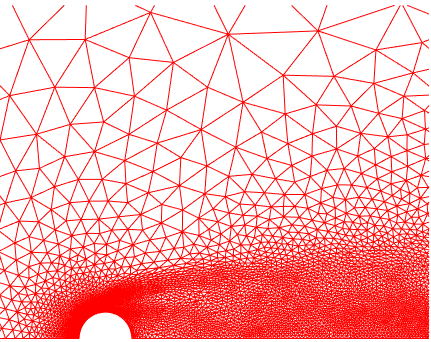
\includegraphics[scale=0.5]{zoom_finner_mesh_final.png}
\end{center}




\vspace{0.35\textheight} % Whitespace between the title block and the publisher
{\noindent IMFT, v0.2 May 2018  }\\[\baselineskip] 
}}
\endgroup}

 % Sets margins and page size
\pagestyle{empty} % Removes page numbers
\makeatletter % Need for anything that contains an @ command 
\renewcommand{\maketitle} % Redefine maketitle to conserve space
{ \begingroup \vskip 10pt \begin{center} \Huge {\bf \@title}
	\vskip 10pt \large \@author \hskip 20pt \@date \end{center}
  \vskip 10pt \endgroup \setcounter{footnote}{0} }
\makeatother % End of region containing @ commands


%\let\vaccent=\v % rename builtin command \v{} to \vaccent{}

\usepackage{cancel}

 %\pagestyle{myheadings}
 
 \begin{document}
 \let\cleardoublepage\clearpage
\titleGM


\tableofcontents

\setcounter{page}{1}
\clearpage

%The chapters

\section*{Previous Note}

\ti{StabFem} is a software to perform Global Stability calculations in Fluid Mechanics, which is developed for both research and education purposes. It can be downloaded at \url{https://github.com/erbafdavid/StabFem}. Additionally, one will previously need to install \ti{Matlab} and \ti{FreeFem++} on the running system. For now, \ti{StabFem} works perfectly in \ti{Ubuntu16.06}. On other Operating Systems, it's not sure that it will work.


This document is a collaboration of different people and is intended to explain, the best way possible, the different parts of \textit{StabFem}. Perhaps as the reader will read it, some chapters are uncompleted or complicated to understand. The reader is invited to contribute in order to render the documentation more understandable.



\clearpage

\chapter{General View of \ti{StabFem}}



\ti{StabFem} has a main directory where all the projects are located and where the mutual scripts are located too. The directory is composed by the following particular project directories:


\begin{enumerate}
\item CASE\_STABLE/ACOUSTICS\_PIPES;
\item CASE\_STABLE/CYLINDER;
\item CASE\_STABLE/CYLINDER\_VIV;
\item CASE\_STABLE/DISK\_IN\_PIPE.
\item etc...
\end{enumerate}
The mutual directories are the followings:

\begin{enumerate}
\item SOURCES\_FREEFEM;
\item SOURCES\_MATLAB;
\item Documentation.
\end{enumerate}

These directories are used by the several projects of \ti{StabFem}.

\medskip

\begin{leftbar}
Attention: When you do some change in the mutual directory files, we have to assure that it will work on all the projects.
\end{leftbar}
\section{General Features}

\begin{itemize}
\item With \ti{StabFem} we can solve forced problems, eigenvalue problems, etc...

\item  \ti{StabFem} allows us to save the scripts used to generate the different data and graphs, unabling to reproduce the same results (useful for repeat figures for articles, confirming results, etc...).
\end{itemize}



\section{What is attended from this manual document}
This document presents this first chapter describing what can be found in a  \ti{StabFem} project, a chapter describing the running logic of a \ti{StabFem} program and the main common files and a chapter for each project, describing succinctly their running features.


% !TEX root = main.tex

\section{Notes and tips for users and developers}

When contributing to the project you can intervene at two levels:

\begin{itemize}

\item Contributring as a {\em User}  means that you will use the available solvers and drivers for a class of problems already integrated 
in the project. For instance, if you wish to study the wake flow around an elliptical 2D body, which uses the same solvers than the case of a circular cylinder already present in the base. 

In this case, you will create a directory for your case (for instance {\em ELLIPSE/}) containing : The mesh generator freefem script 
(for instance {\em Mesh\_Ellipse.edp}), the macro file {\em Macros\_Stabfem.edp}  containing the case-dependent boundary condition and postprocessing detail, and a number of Mablab scripts. O,n the other hand, you will suposedly not modify thecommon files in the source directories (with the exception of the file {\em SOURCES\_MATLAB/SF\_Start.m}).

\item Contributing as a {\em Developer } means that you wish to help integrate new Freefem solver into the project 
(for instance, you want to solve a 2D problem in the Bousinesq approximation, you already have a set of Freefem solvers for this case and you wish to integrate them in the project).

\end{itemize}

 
\subsection{FAQ}
 
 
 
Here is a kind of FAQ of the projecft, regerouping in random order notes, tips and "good practize recomendations" for users and developers.
 


\begin {itemize}

\item
At installation (git clone) it is recommended that you install the whole StabFem project in your home directory and that you do
not remove or displace the parts of the project that you don't (immediately) need. Otherwise this will perturb the operation of the version manager git. 
In short :  if you there are parts you think you don't need, don't remove them, just ignore them !


\item good usage of the "verbosity"' parameter ...


\end{itemize}

\subsection{Note on the usage of github}
  
The project is supported by the git subversion manager program. Here are a fexw tips/recommendations :

\paragraph{If you are contributing as a user}

\begin {itemize}

\item After the initial git clone, you may want to get the latest development of the main branch using {\em git pull}. This will only update the sources in the common repositories, not your own files. 

If you have modified the {\em SF\_Start.m} file and/or made minor modifications to other files that you wish to keep in your local version but do not want to export to the main branch odf the project, the procedure is to do successively :

git stash

git pulll

git stash apply.

(don't be afraid, any "mistake" with git can be undone !) 

\item 
If you want to incorporate your work in the project repository (normally after everything is validated...) you should do the following :

git add "files".  {\em (please add only source files of your case directory, such as freefem mesh generator and macro scripts, an example matlab script producing sample results for your case, and possibly matlab functions you have developed for your own case and are not sure they will work for other cases)}


git commit -a

git push

{\em For this last step you need to be register as a contributor, just ask !}




\item (...)

\end{itemize}


\paragraph{If you are contributing as a developer}

\begin {itemize}

\item The best way is to creat a "fork" or a "branch" (still not sure what is the most efficient)

\item Once you have your own branch/fork, use gut commit / git push as frequently as you wish !

\item If you want to merge with the main branch, create a {\em pull request}.

\item (...)

\end{itemize}

\section{Notes/tips about FreeFem}

All the Freefem tricks which are not in the manual....







\clearpage

\part{Stabfem principles : learning by examples}


% !TEX root = main.tex

\chapter{The basics of StabFem }


In this chapter we explain the basic functionalities of StabFem. We recommend that you study the basic example \keys{EXAMPLE\_Lshape.m}.

This directory contains three freefem programs and a demo matlab script doing solving the following problem :


\section{Simple problem : solution of heat equation in a L-shaped domain}

1. Solve the steady heat conduction equations on a L-shaped domain with constant volumic source term $P$ and homogeneous Dirichlet boiundary conditions :

$$ \nabla^2 T = P  \mbox {  for } {\bf x} \in \Omega ; \quad T = 0   \mbox {  for } {\bf x} \in \Gamma$$

2.  Solve the unsteady heat conduction equations on a L-shaped domain with zero source term $P$ and time-periodic Dirichlet boundary conditions :

$$ 
 \partial T_1/\partial t= \nabla^2 T_1  \mbox {  for } {\bf x} \in \Omega ; \quad T_1 = T_w e^{i \omega t}   \mbox {  for } {\bf x} \in \Gamma
$$



\section{Matlab script and results}

The programs are sufficiently short to be fully given in these pages. See figures \ref{SCRIPT_Lshape.m},  \ref{Lshape_Mesh.edp}, \ref{Lshape_Steady.edp}.  

The reader already familiar with FreeFm++ should not have any provblem in undersanding the programs. If not, we recommand that you study the FreeFem++ Manual (chapter "Learning by examples").

The results are given in figure \ref{Lshape_Figures}.



\begin{figure*}[t]
\small
\lstinputlisting{../EXAMPLE_Lshape/SCRIPT_Lshape.m}
 \normalsize
\caption{
Matlab program \keys{SCRIPT\_Lshape.m})}
\label{SCRIPT_Lshape.m}
\end{figure*}


\begin{figure*}[t]
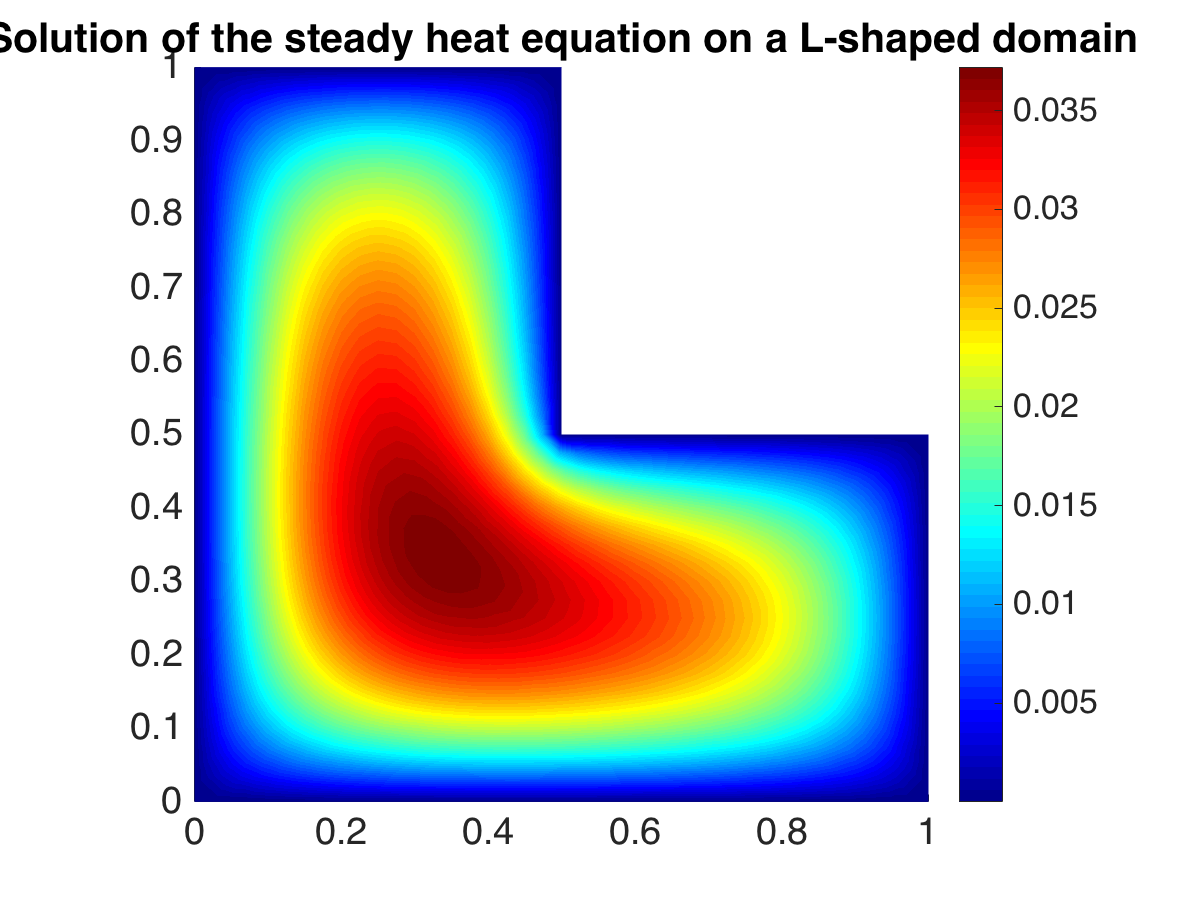
\includegraphics[width = .45 \linewidth]{../EXAMPLE_Lshape/FIGURES/Lshape_T0.png}
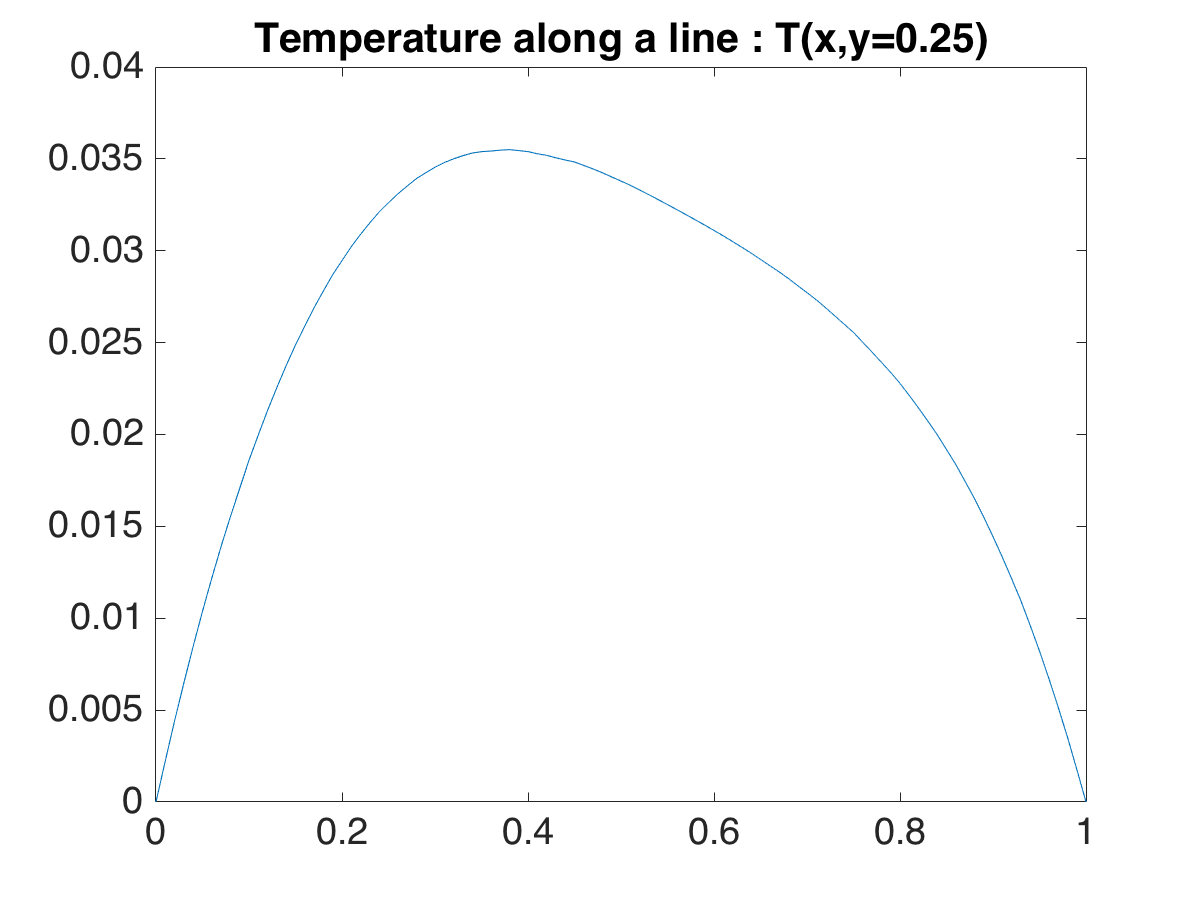
\includegraphics[width = .45 \linewidth]{../EXAMPLE_Lshape/FIGURES/Lshape_T0_Cut.png}
\caption{Solution for the steady hrat equation in a L-shape domain : $(a)$ Temperature field $T(x,y)$. 
$(b)$ Temperature $T(x,0.25)$ along a horizontal line. }
\label{Lshape_Figures}
\end{figure*}

\begin{figure*}[t]
\small
\lstinputlisting{../EXAMPLE_Lshape/Lshape_Mesh.edp}
 \normalsize
\caption{
FreeFem++ program \keys{Lshape\_Mesh.edp})}
\label{Lshape_Mesh.edp}
\end{figure*}


\begin{figure*}[t]
\small
\lstinputlisting{../EXAMPLE_Lshape/Lshape_Steady.edp}
\normalsize
\caption{
FreeFem++ program \keys{Lshape\_Steady.edp})}
\label{Lshape_Mesh.edp}
\end{figure*}


\clearpage

%%%%%%%%%%%%%%%%%%%%%%%%%%%%%%%%%%%%%%%%%%%%%%%
\section{How does it work ?}

\subsection{Analysis of the example}

Let us observe and explain the most important steps of the example matlab script \keys{SCRIPT\_Lshape.m}. 

\begin{itemize}
\item  The first step is {\bf creating and importing a mesh}. This is done by the function \keys{SF\_Mesh.m} invoked at line 7 of the script. 
Basically this function does the following operations :
\begin{enumerate}
\item Launch the FreeFem++ program \keys{Lshape\_Mesh.edp} with the {\em entry parameter} \footnote{Here and in the sequel, 
{\em entry parameter} means a value you will be invited to type on the keyboard if using directly FreeFem++ in the way you are used to. Just try !}
$Ndensity = 40$ (here corresponding to the mesh density).
\item Import the data produced by the FreeFem++ Macro {\sf SFWriteMesh} (more explanations in paragraph 3.3) 
\item Return the data as a Matlab {\em structure} object called {\sf ffmesh}
\end{enumerate}

Execution of this step leads to the following :
\lstinputlisting[linerange={1-15}]{Lshape_ExecutionExample.txt}

This structure objects has several fields which will serve for plotting data obtained on this mesh. See more in section 2.3.

\item The second step is {\bf launching a FreeFem program using this mesh and importing results}. 
This is done by the generic driver function \keys{SF\_Launch.m} invoked at line 12 of the script. 
Basically this function does the following operations :
\begin{enumerate}
\item Launch the FreeFem++ program \keys{Lshape\_Steady.edp}  (here with no {\em entry parameter}).
\item Import the data produced by the FreeFem++. By default the driver will look for a file called \keys{Data.ff2m}. 
This file is the one created by the FreeFem program in lines 14-22 of the Freefem program \ref{Lshape_Steady.edp}.

Looking inside the file \keys{Data.ff2m}, the header (i.e.  first four lines) is as follows :
\lstinputlisting[linerange={1-5}]{../EXAMPLE_Lshape/Data.ff2m}, 
meaning that this files contains a P1 mesh-organised field called 'T'.

\item Return the data as a matlab {\em structure} object called {\sf heatS}.
\end{enumerate}

Execution of this step leads to the following :
\lstinputlisting[linerange={17-24}]{Lshape_ExecutionExample.txt}

Where we can see that the structure has field called 'T' (containing the imported data)
 and a field called 'mesh'  which is actually the mesh object previously constructed and passed to the driver as a parameter as a field.


\item The third step which is important to explain ist {\bf importation of results previously generated by Freefem}. 
This is done by the generic driver function \keys{importFFdata.m} invoked at line 12 of the script. 

Here, besides the file Data.edp previously imported, our program has generated a second data file called \keys{Heat\_1Dcut.ff2m}.
%This file is the one created by the FreeFem program in lines 14-22 of the Freefem program \ref{Lshape_Steady.edp}.
The header of this file is as follows :
\lstinputlisting[linerange={1-5}]{../EXAMPLE_Lshape/Heat_1Dcut.ff2m}, 
meaning that this files contains two vectors of dimension 101 called X and T.


Execution of this step leads to the following :
\lstinputlisting[linerange={26-32}]{Lshape_ExecutionExample.txt}


Where we can see that the data is imported as a structure with two fields corresponding to the required data.

\end{itemize}

The \keys{importFFdata.m} functions is the core of the interface, and is actually internally called by the higher-levels drivers \keys{SF\_Mesh.m}  and \keys{SF\_Launch.m}.

 
%\caption{
%File \keys{Data.ff2m})}
%\label{Lshape_Data.ff2m}
%\end{figure*}

%File \keys{Heat\_1Dcut.ff2m}

%\lstinputlisting[linerange={1-5}]{../EXAMPLE_Lshape/Heat_1Dcut.ff2m}


%\lstinputlisting{../EXAMPLE_Lshape/ExecutionExample}

\subsection{Explanations of the \texttt{.ff2m} exchange format}


As can be seen in the previous short examples, the basis of the FreeFem/Matlab interface relies in the file exchange format \keys{.ff2m}
and the importation "wizard"  \keys{importFFdata.m} which reads these files.

Let us explain how such files are constituted. As we have observed, the header of a \keys{.ff2m} file has the following structure :

\lstinputlisting{Lshape_FormatExplanation.ff2m}.

The line 4 explains the nature of the data which is contained in the file.
There can be as many data objects as you want organised in the order of your choice. The recognized types are currently as follows :
\begin{description}
\item{ \bf P1}  for mesh-structured data stored as P1 finite-elements
\footnote{P2 data is not yet supported, the solution is to convert everything to P1 before exportation.}  
\item{\bf P1c}  for mesh-structured {\em complex} data stored as P1 finite-elements
\item{\bf real} for real scalars,
\item{\bf complex} for complex scalars,
\item{\bf real.N} for real vectors of dimension N not associated to a mesh,
\item{\bf complex.N} for complex vectors of dimension N not associated to a mesh,
\item{\bf P1s} for real data defined along a frontier of the mesh,
\item{\bf P1sc} for complex data defined along a frontier of the mesh.
\end{description}

\subsection{Explanations about the mesh }

to be continued...








% !TEX root = main.tex

\chapter{Using StabFem for globals stability calculations}

The stabfem software was initially designed to perforrm global stability calculations (linear and nonlinear).
This chapter explains this throufh the example of the wake of a cylinder.

The theory is fully explained in the submitted paper [...]. In this chapter we explain the implementation issues.




{\em 
Newt of the chapter is initial version of Diogo,n to be recast)
}


A \ti{StabFem} project have a directory, for example \directory{StabFemm>CYLINDER} where it can be found: 
\begin{enumerate}
\item The \texttt{*.m} files corresponding to the \ti{Matlab} scripts. Normally, a main script can be found, e.g. \keys{SCRIPT\_CYLINDER\_DEMO.m} ;
\item A directory \directory{StabFemm>CYLINDER > WORK} (if not, it will be created when \ti{Matlab} script run) where it can be found the output data;
\item All the \texttt{*.edp} specific to the project and to be editexecuted automatically by the \ti{Matlab} interface. E.g.: The \keys{Mesh*.edp}, the \keys{Macros\_StabFem.edp}, \keys{Param\_Adaptmesh.edp}, etc.
\end{enumerate}



\section{Running logic of a \ti{StabFem} project}


When one executes the main script \texttt{*.m}, both local and share scripts are executed. For a commum project, the following steps done:

\begin{enumerate}
\item Launch the share script \keys{SF\_Start.m}:
\begin{lstlisting}
run('../SOURCES_MATLAB/SF_Start.m');
\end{lstlisting}
creating the following directories as global variables and adding the \ti{sfdir} to the \ti{matlab} paths:
\begin{lstlisting}
ff = '/PRODCOM/Ubuntu16.04/freefem/3.51/gcc-5.4-mpich_3.2/bin/FreeFem++'; % on IMFT network
sfdir = '~/StabFem/SOURCES_MATLAB/'; % where to find the matlab drivers
ffdir = '~/StabFem/SOURCES_FREEFEM/'; % where to find the freefem scripts
ffdatadir = './WORK/';
addpath(sfdir);
\end{lstlisting}
It also creates the \keys{SF\_Geom.edp} need for \ti{FreeFemm++}.


\item Then, a mesh and a baseflow are generated for the project with the help of the share script \keys{SF\_Init.edp} located in \directory{StabFemm>SOURCES\_MATLAB},e.g.:

\begin{lstlisting}
baseflow=SF_Init('Mesh_Cylinder.edp', [-40 80 40]);
\end{lstlisting}

The detailed input/output parameters are discussed in next chapter (\textcolor{red}{To do...}). It will execute \keys{Mesh*.edp} and generate in the current path the \keys{mesh.msh}, \keys{mesh.ff2m}, \keys{mesh\_init.msh},\keys{SF\_Init.ff2m}, \keys{BaseFlow\_init.txt} and \keys{BaseFlow\_init.ff2m} files. 

The path \directory{StabFemm>CYLINDER > WORK>BASEFLOWS} is created. This is where all the base flow for the different Reynolds numbers will be stored.



\item The baseflows for for different parameters ($Re$, Porosity,...) are generated by the command: 
\begin{lstlisting}
baseflow=SF_BaseFlow(baseflow,'Re',10);
\end{lstlisting}
executing the commom scritpt \keys{SF\_BaseFlow.m}. This script will read the \ti{baseflow.mesh.problemtype} parameter and execute the corresponding Newton routing \texttt{Newton*.edp} located at \directory{StabFemm>SOURCES\_FREEFEM} in order to generate the corresponding baseflows in their path.


\item Then, a adaptation of the mesh is made to refine and converge the results for the correct baseflow, with the following command:
\begin{lstlisting}
baseflow=SF_Adapt(baseflow,'Hmax',10,'InterpError',0.005);
\end{lstlisting}
The refine parameters are written in \keys{Param\_Adaptmesh.edp}\textcolor{red}{(why?)} in the current path. \keys{Adapt\_Mode.edp} is executed from \ti{ffdir} to refine the mesh. \textcolor{red}{(Some files are created...explain...)}

\item A mesh adaptation taking into account the eigenmode can be done: for that, first a solution have to be commuted first giving the eigenmodes. Then the mesh adaptation can be done like it was done in last step. 
\begin{lstlisting}
[ev,em] = SF_Stability(baseflow,'shift',0.04+0.74i,'nev',1,'type','D');
[baseflow,em]=SF_Adapt(baseflow,em,'Hmax',10,'InterpError',0.01);
\end{lstlisting}

Here, the eigenvalue problem has been solved with a shitf-and-invert iteration process, detail in next chapter(\textcolor{red}{(to do)}). \keys{SF\_Stability.m} is once again located at \ti{sfdir}.

\item After the former step, once wisely used, post-processing can be made. At that stage, each project have its particularities and it will be detailed in their dedicated chapters.
\end{enumerate}

\section{Create a \ti{StabFem} project}

In order to create a project in \ti{StabFem} one has to start to code the scripts in \ti{FreeFEM++}.

\medskip

\begin{leftbar}
Attention:  When creating the different \texttt{*.edp} files, one has to pay attention on the compulsory inputs and output of the \ti{Matlab} interface.
\end{leftbar}

Then, the \ti{Mathlab} scripts, with the previously presented style, have to be created.

\medskip

\begin{leftbar}
Attention:  The different \texttt{*.m} files created in the particular directory will be used only in your project, so you can used them as you like; but, once the common files are used, they must not be changed without careful examination of the impact on the other projects.
\end{leftbar}


Commonly, the following files are needed in the current file:

\paragraph{\ti{FreeFEM++} file: SCRIPT\_*.edp}

Here, the problem is defined. See chapter \textcolor{red}{(to do)} for more details. It can be a eigenvalue problem, a forced problem, etc. To define the problem, see the FreeFEM++ documentation \cite{FFdoc}\footnote{http://www.freefem.org/ff++/ftp/freefem++doc.pdf}.

\paragraph{\ti{FreeFEM++} file: Mesh\_*.edp}

File where the mesh of the problem and the convenient files are generated.

\paragraph{\ti{FreeFEM++} file: Macros\_StabFem.edp}

Macros are a powerful tool in \ti{FreeFEM++}. In this file all the Macros specific of the project are created. This macros will be used both by the \texttt{*.edp} scripts of one's problem and by the  common scripts located at \directory{StabFemm>SOURCES\_FREEFEM}. 


\paragraph{\ti{Matlab} file: mains\_cript.m}

This script will be organise like in the previously presented style. Then, the a  different treatment is given to each problem, and one can be inspired by the project already created.




% !TEX root = main.tex

\chapter{Using StabFem to perform DNS (tipe-stepping resolution of NS equations)}

Not yet implemented but coming very soon...

         
\input{14_StabFem_Plotting.tex}  


\clearpage


\part{Description of the test-cases}

% !TEX root = main.tex

\chapter{Stability of the flow around a 2D cylinder}

\begin{description}
\item{Directory in the StabFem project :}  \texttt{CYLINDER}
\item{Main contributors :} D. Fabre, V. Citro, D. Ferreira-Sabino
\item{Reference :} A practical review on linear and nonlinear global approaches to stability analysis, D. Fabre et al., {\em submitted to Rev. Appl. Mech (2018)}
\end{description}
% !TEX root = main.tex

\chapter{Stability of the flow around a spring-mounted}

\begin{description}
\item{Directory in the StabFem project :}  \texttt{CYLINDER\_VIV}
\item{Main contributors :} Diogo
\item{Reference :} 
\end{description}

% !TEX root = main.tex

\chapter{Stability of the flow around a flying menhir}

\begin{description}
\item{Directory in the StabFem project :}  \texttt{MENHIR}
\item{Main contributors :} Obelix \& Cie.
\item{Reference :} Asterix et le coup du menhir, R. Goscinny \& A. Udezo. Dargaud Ed.  
\end{description}

% !TEX root = main.tex

\chapter{Capillary oscillations of a liquid bridge}

\begin{description}
\item{Directory in the StabFem project :}  \texttt{LiquidBridges}
\item{Main contributors :} D. Fabre.
\item{Reference :} Chireux et al., Phys. Fluids, 2015.
\end{description}


\begin{figure}
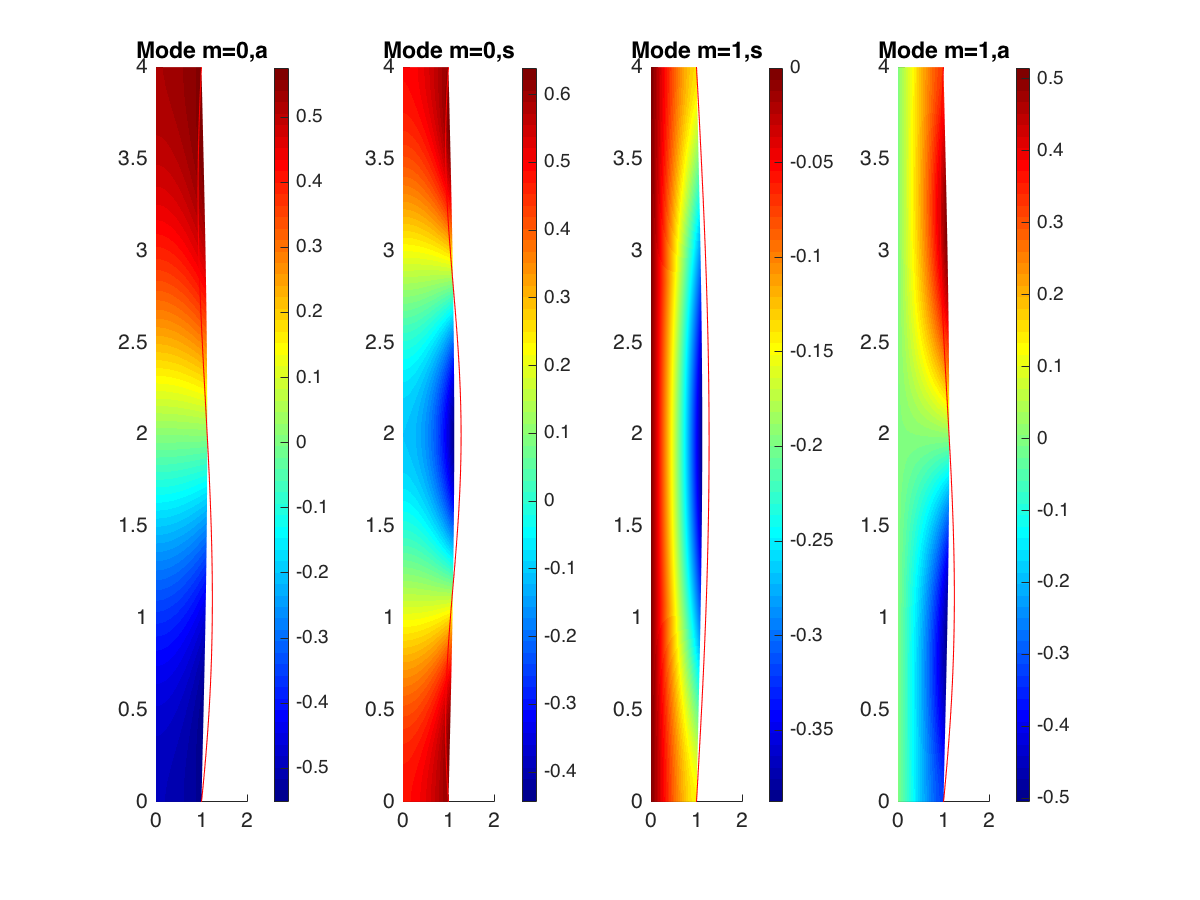
\includegraphics[width=.8\linewidth]{../../CASES_STABLE/LiquidBridges/FIGURES/Bridges_NV_Eigenmodes_phi_cyl_L3_5.png}
\caption{Oscillation modes of a liquid bridge of aspect ratio $L/R=4$ and reduced volume $V^ =$...}
\label{Bridges_NV_Eigenmodes_phi_cyl_L3_5}
\end{figure}

\begin{figure}
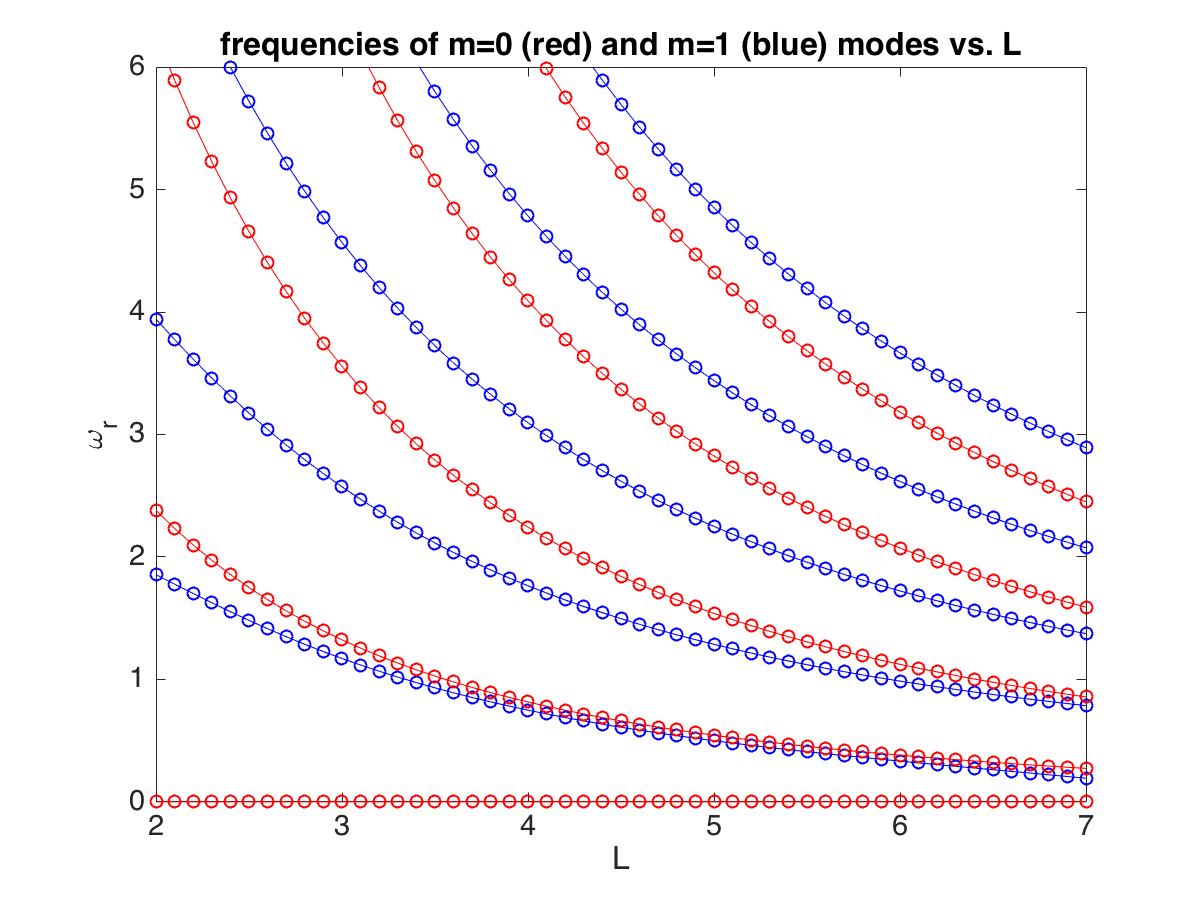
\includegraphics[width=.45\linewidth]{../../CASES_STABLE/LiquidBridges/FIGURES/Bridges_NV_coal_omega.png}
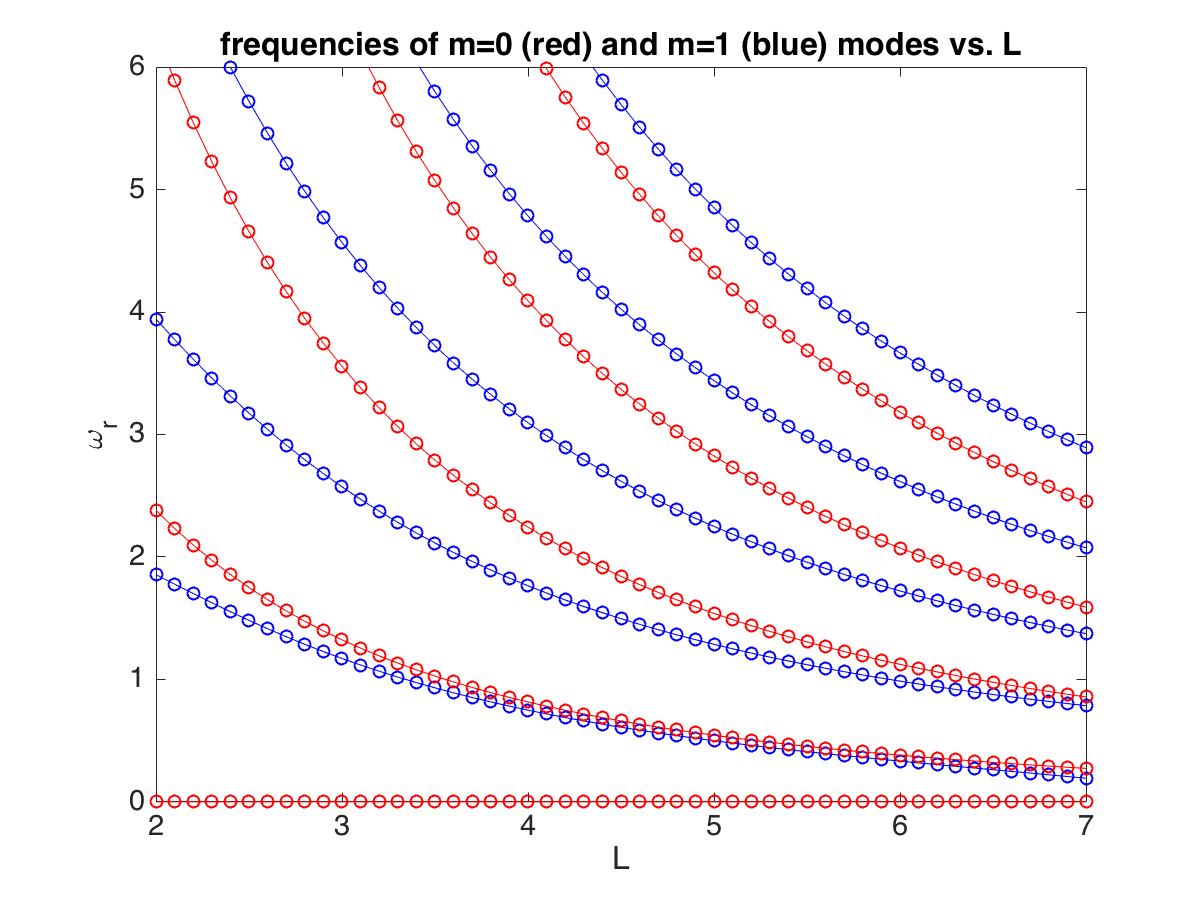
\includegraphics[width=.45\linewidth]{../../CASES_STABLE/LiquidBridges/FIGURES/Bridges_NV_coal_omega.png}
\caption{Oscillation frequencies of a liquid bridge resulting from the coalescence of two spherical droplets
as function of $L^* =L/R$
(figures 11,12 of Chireux et al.)
}
\label{Bridges_NV_Eigenmodes_phi_cyl_L3_5}
\end{figure}
 
% !TEX root = main.tex

\chapter{Instabilities of a potential free-surface vortex flow}

\begin{description}
\item{Directory in the StabFem project :}  \texttt{ROTATINGPOLYGONS}
\item{Main contributors :} J. Mougel, D. Fabre
\item{Reference :} Mougel et al., JFM 2018 
\end{description}

\begin{figure}
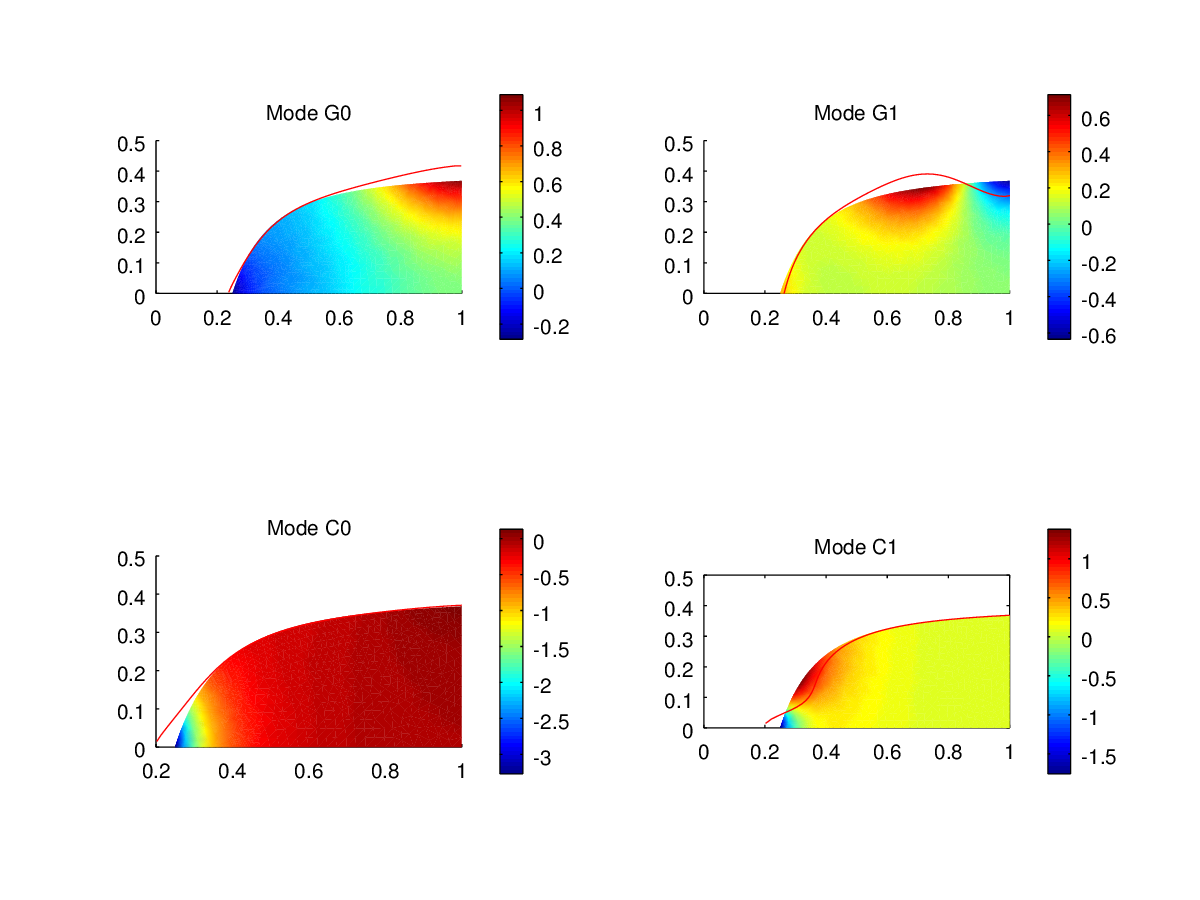
\includegraphics[width=.8\linewidth]{../../CASES_STABLE/ROTATING_POLYGONS/FIGURES/POLYGONS_modes.png}
\caption{Oscillation modes of a potential vortex for  $a=H/R=0.3$ and $m=3$ (figure 5, 6 of Mougel et al.).}
\label{Bridges_NV_Eigenmodes_phi_cyl_L3_5}
\end{figure}

\begin{figure}
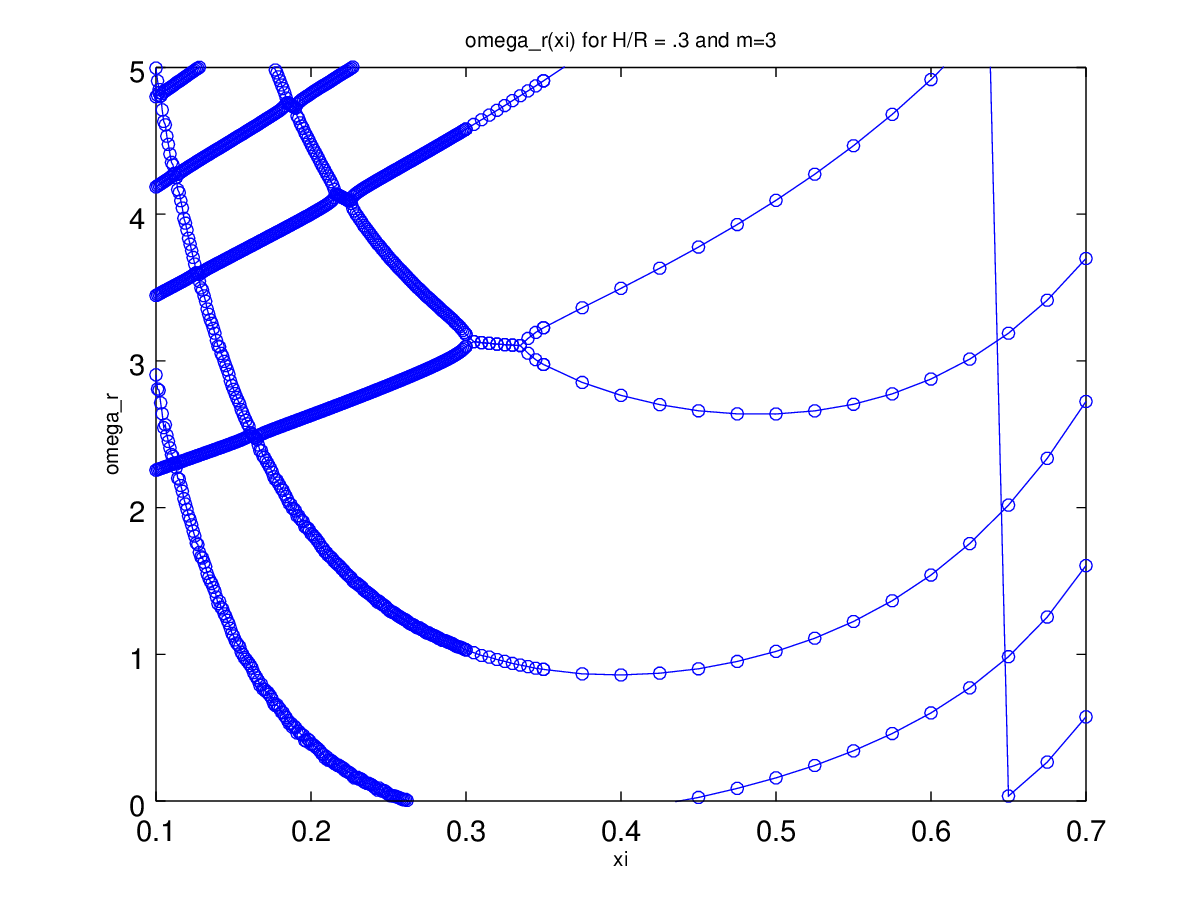
\includegraphics[width=.45\linewidth]{../../CASES_STABLE/ROTATING_POLYGONS/FIGURES/POLYGONS_omega.png}
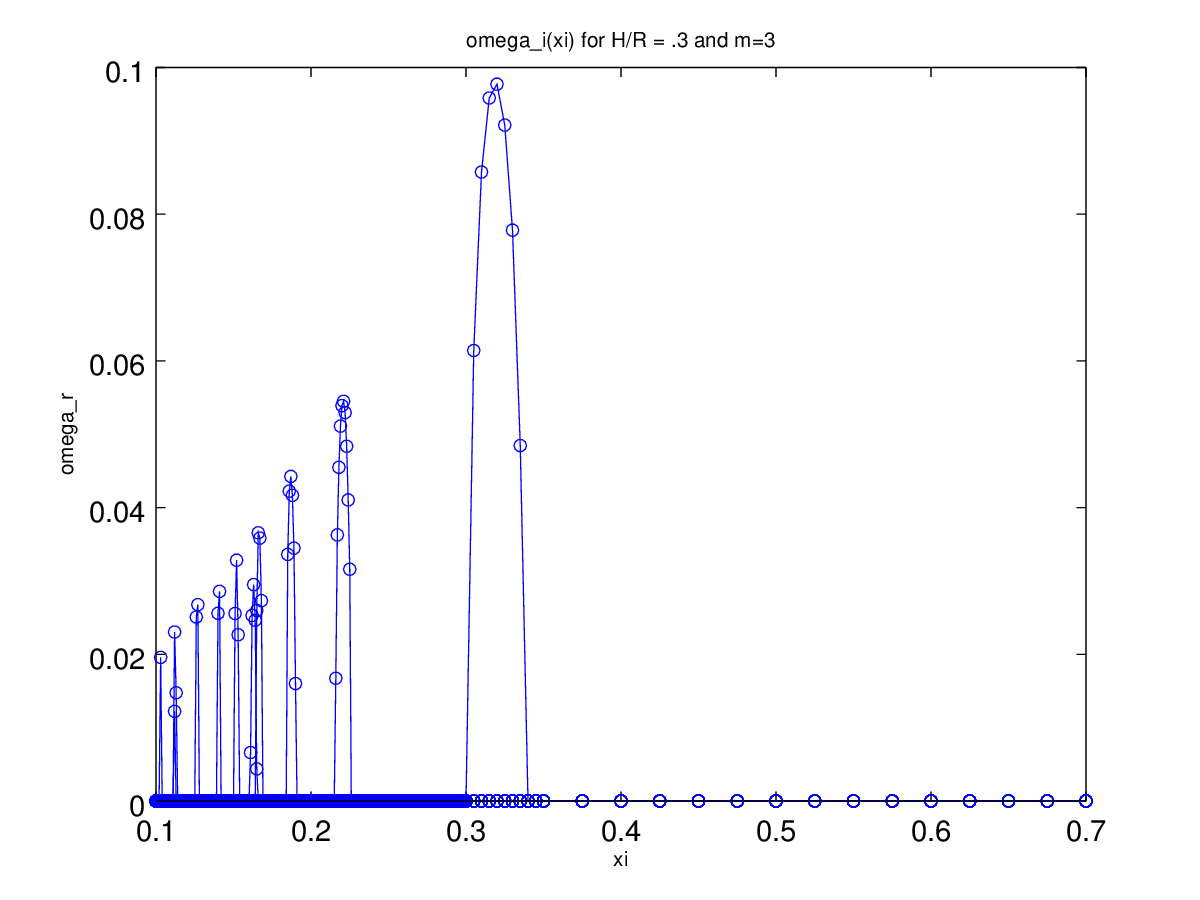
\includegraphics[width=.45\linewidth]{../../CASES_STABLE/ROTATING_POLYGONS/FIGURES/POLYGONS_sigma.png}
\caption{Oscillation frequencies and amplification rates for f a potential vortex for $m=3$ (figure 4 of Mougel et al.).}
\label{Bridges_NV_Eigenmodes_phi_cyl_L3_5}
\end{figure}
 

\appendix

\part{Appendix : documentation of the source programs}


% !TEX root = main.tex
\chapter{Mutual Matlab Files}

In this section we give the documentation of the Matlab drivers of the project.

We have to find a way to generate automatically this documentation by extracting the documentation directly from the programs
(Doxygen ?)


\section{General drivers and FF/Matlab interface tools}

\subsection{\texttt{SF\_Mesh.m}}

\subsection{\texttt{SF\_Launch.m}}

\subsection{\texttt{importFFMesh.m}}

\subsection{\texttt{importFFData.m}}


\section{Stability-oriented drivers}

\subsection{\texttt{SF\_Init.m}}

\subsection{\texttt{SF\_BaseFlow.m}}

\subsection{\texttt{SF\_Stability.m}}

\subsection{\texttt{SF\_Adapt.m}}

\section{Plotting programs}



\section{Auxiliary programs}

\subsection{\texttt{mysystem.m}}

\subsection{\texttt{mycp.m}}



%\clearpage

\input{302_Mutual_Files_FreeFEM.tex}
%\clearpage

%\input{06_problem_definition.tex} to create
%\clearpage

%\section{Cylinder VIV project}
%\clearpage


%%%%%%%%%%%%%%%%%%%%%%%%%%%%%%%%%%%%%%%%%%%%%%%%%%%%%%%
%Bibliographie
\clearpage
\bibliographystyle{plain}
\bibliography{98_Biblio.bib}
\end{document}